\documentclass[9pt]{beamer}

%~~~~~~~~~~~~~~~~~~~~~~~~~~~~~~~~~~~~~~~~~~~~~~~~~~~~~~~~~~~~~~~~~~~~~~~~~~~~~~
% Use roboto Font (recommended)
\usepackage[sfdefault]{roboto}
\usepackage[utf8]{inputenc}
\usepackage[T1]{fontenc}
%~~~~~~~~~~~~~~~~~~~~~~~~~~~~~~~~~~~~~~~~~~~~~~~~~~~~~~~~~~~~~~~~~~~~~~~~~~~~~~

%~~~~~~~~~~~~~~~~~~~~~~~~~~~~~~~~~~~~~~~~~~~~~~~~~~~~~~~~~~~~~~~~~~~~~~~~~~~~~~
% Define where theme files are located. ('/styles')
\usepackage{styles/fluxmacros}
\usefolder{styles}
% Use Flux theme v0.1 beta
% Available style: asphalt, blue, red, green, gray 
\usetheme[style=green]{flux}
%~~~~~~~~~~~~~~~~~~~~~~~~~~~~~~~~~~~~~~~~~~~~~~~~~~~~~~~~~~~~~~~~~~~~~~~~~~~~~~

%~~~~~~~~~~~~~~~~~~~~~~~~~~~~~~~~~~~~~~~~~~~~~~~~~~~~~~~~~~~~~~~~~~~~~~~~~~~~~~
% Extra packages for the demo:
\usepackage{booktabs}
\usepackage{colortbl}
\usepackage{ragged2e}
\usepackage{schemabloc}
\usepackage{subfigure}
\usepackage{hyperref}
\usepackage[usenames]{color}
%~~~~~~~~~~~~~~~~~~~~~~~~~~~~~~~~~~~~~~~~~~~~~~~~~~~~~~~~~~~~~~~~~~~~~~~~~~~~~~
%~~~~~~~~~~~~~~~~~~~~~~~~~~~~~~~~~~~~~~~~~~~~~~~~~~~~~~~~~~~~~~~~~~~~~~~~~~~~~~
% Informations
\subtitle{\\
\LARGE{Predicción del comportamiento de una enfermedad} \\
\LARGE{simulada en autómatas celulares con un algoritmo}\\
\LARGE{propuesto en redes neuronales}}
%\subtitle{The winding number}
\author{Jorge Andres Ibañez Huertas}
\institute{Central University, Bogotá}
\date{\today}
\titlegraphic{Imagenes/logo.png}
%~~~~~~~~~~~~~~~~~~~~~~~~~~~~~~~~~~~~~~~~~~~~~~~~~~~~~~~~~~~~~~~~~~~~~~~~~~~~~~

\begin{document}

% Generate title page
\titlepage

\begin{frame}
\frametitle{Tabla de Contenidos}
\tableofcontents
\end{frame}

\section{Estudio epidemiológico}\label{sec:Estudio epidemiológico}
\begin{frame}{El Estudio Epidemiológico}
\textbf{La epidemiología}

De acuerdo con \cite{epiDictionary}, la epidemiología se encarga de estudiar la ocurrencia y distribución de eventos, estados y procesos relacionados con la salud de distintas poblaciones, con el objetivo de brindar estrategias de control y prevención de problemas de salud relevantes.

Uno de los objetos de estudio con mayor importancia en el campo de la epidemiología es la cualidad endémica de la enfermedad. La manera en la que se determina está capacidad está dada por los siguientes indicadores:

\begin{itemize}
    \item \textbf{Número básico de reproducción $R_0$:} Se define como la cantidad de individuos que infecta el paciente cero en una población completamente susceptible.
    \item \textbf{Número de contactos adecuados $\sigma(t)$:} Es la cantidad de contactos con individuos del sistema que realiza un individuo infectado durante su etapa de infección, cuando se introduce en la población en el momento $t$.
    \item \textbf{Número de desplazamiento $R(t)$:} Se entiende como la cantidad promedio de infecciones secundarias que produce un individuo infectado durante su etapa de infección, cuando es introducido en la población en el momento $t$.
\end{itemize}
\end{frame}

\begin{frame}{El Indicador $R_0$}
Heesterbeek y Dietz definen el número básico de reproducción $R_0$ como

\begin{equation}\label{eq:R0}
    R_0 = \int_0^\infty b(a)F(a) da
\end{equation}

donde $b(a)$ representa la cantidad promedio de nuevos contagios que producirá un individuo infectado durante un tiempo y $F(a)$, conocida como la función de supervivencia, representa la probabilidad de que un individuo recién infectado se mantenga en ese estado durante al menos un tiempo $a$ \cite{conceptOfR0, perspectivesOnR0}.

\begin{alertblock}{Observación}
En general, si $R_0<1$ la enfermedad desaparecerá paulatinamente y sí $R_0>1$, podríamos estar ante un caso de endemia.
\end{alertblock}
\end{frame}

\section{Modelos epidemiológicos clásicos}\label{sec:Modelos epidemiológicos clásicos}
\begin{frame}{Modelos epidemiológicos clásicos}
Tradicionalmente, se han utilizado modelos de compartimientos para elaborar análisis epidemiológicos. En estos modelos, cada individuo perteneciente a la población de estudio es clasificado en uno de $n$ posibles estados, según su estado de salud.\cite{modelCompartimental}

\begin{figure}[h]
  \centering
    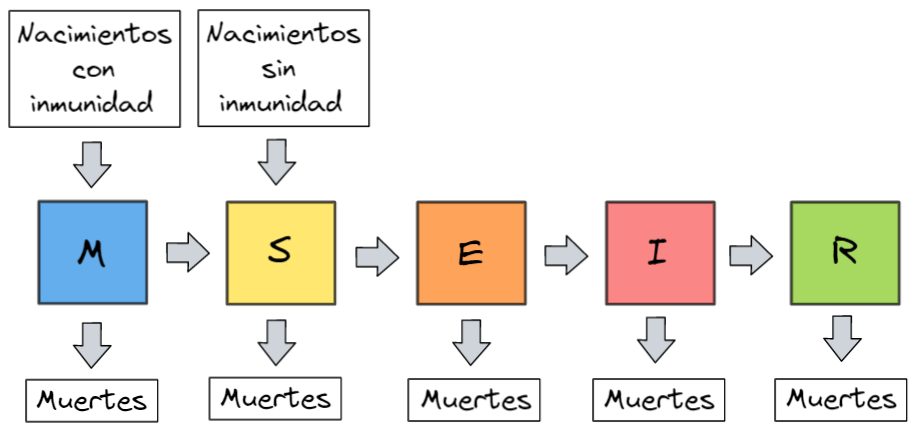
\includegraphics[width=0.7\textwidth]{Imagenes/MSEIR_compatimientos.PNG}
  \caption{Diagrama de compartimientos para el modelo MSEIR}
  \label{fig:diagrama MSEIR}
\end{figure}
\end{frame}

\subsection{El modelo SIS}\label{sub:El modelo SIS}
\begin{frame}{El Modelo SIS}
Las variaciones entre los estados vienen dadas por los nuevos contagios y los individuos que se recuperan de la enfermedad. Adicionalmente, cada estado se ve afectado por los parámetros que describen la natalidad/mortalidad y la muerte a cauda de la enfermedad. 

\begin{figure}[h]
  \centering
    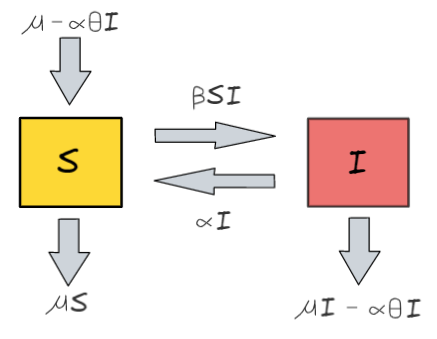
\includegraphics[width=0.4\textwidth]{Imagenes/SIS_compartimientos.PNG}
  \caption{Diagrama de compartimientos para el modelo SIS}
  \label{fig:diagrama SIS}
\end{figure}

Trabajaremos sobre una población de tamaño constante y normalizado, por lo que $S + I = 1$ y en consecuencia $S' + I' = 0$.
\end{frame}

\begin{frame}{El Modelo SIS}
Podemos describir el modelo a partir de un sistema de ecuaciones diferenciales como sigue:

\begin{equation}\label{eq:Modelo SIS}
\left\{
\begin{array}{l}
S' = \mu(1 - S) + (1 - \theta)\alpha I - \beta S I \\
I' = \beta S I - (1 - \theta)\alpha I - \mu I
\end{array}
\right.
\end{equation}

Para determinar el valor de $R_0$ se considera una población completamente susceptible, es decir, $S=1$ y $I=0$.

Observe que los nuevos infectados vienen dados por el término $\beta S$, con lo cual definimos $b(t) = \beta S = \beta$. Por otro lado, los flujos que determinan la salida del estado de infección de los individuos viene dado por los términos $-\alpha(1-\theta)I-\mu I$, de modo que si llamamos $I(t)$ a la cantidad de individuos infectados que permanecieron infectados desde el momento 0, tenemos
\end{frame}

\begin{frame}{El Modelo SIS}

\begin{equation}\label{eq:Cambio en I}
\frac{dI}{dt} = -\alpha(1-\theta)I-\mu I \Longrightarrow I(t) = I(0)e^{-(\alpha(1-\theta)+\mu)t} \Longrightarrow F(t) = e^{-(\alpha(1-\theta)+\mu)t}
\end{equation}

Finalmente, al reemplazar en (\ref{eq:R0}) obtenemos:

\begin{align*}
R_0 &= \lim_{T\to\infty}\int_0^T b(t)F(t) dt \\
&= \lim_{T\to\infty}\int_0^T \beta e^{-(\alpha(1-\theta)+\mu)t} dt\\
&= \frac{\beta}{\alpha(1-\theta)+\mu}
\end{align*}
\end{frame}

\begin{frame}{Estudio Numérico - El Método de Euler}
De manera general, dadas unas condiciones iniciales $S(0)=S_0,I(0)=I_0$ aplicamos el método de Euler a partir de la siguiente expresión

$$\left\{\begin{array}{l}
S_{t+1} = S_t + h\cdot(\mu(1 - S_t) + (1 - \theta)\alpha I_t - \beta S_t I_t ) \\
I_{t+1} = I_t + h\cdot(\beta S_t I_t - (1 - \theta)\alpha I_t - \mu I_t)
\end{array}\right.$$
\begin{itemize}
    \item Consideremos por ejemplo una enfermedad en la que la tasa de recuperación $\alpha$ es del $0.2$ y su tasa de infección es de $\beta=0.5$ con una tasa de letalidad de $\theta=0.4$. La tasa de natalidad para nuestra población será de $\mu=\frac{1}{75\cdot365}$, es decir, una esperanza de vida de $75$ años.
    
    \begin{figure}[h]
      \centering
        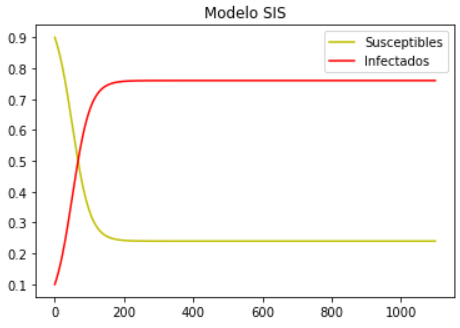
\includegraphics[width=0.4\textwidth]{Imagenes/ex1SIS.PNG}
      \caption{Evolución de la enfermedad en 1100 días con $S_0=0.9,I_0=0.1$ y $h=0.1$.}
      \label{fig:Ejemplo 1 - SIS}
    \end{figure}
\end{itemize}
\end{frame}

\subsection{El modelo SIR}
\begin{frame}{El Modelo SIR}
Para este modelo se considera el estado de inmunidad frente a la enfermedad R. A diferencia del modelo SIS, en el modelo SIR no hay una interacción del estado I al estado S, ya que se supone que los individuos que se recuperen de la enfermedad no podrán volver a contraerla, por lo que pasaran al estado R. 

\begin{figure}[h]
  \centering
    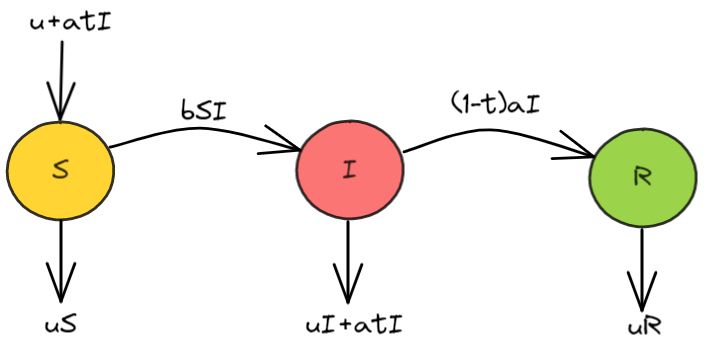
\includegraphics[width=0.7\textwidth]{Imagenes/SIR_compartimientos.PNG}
  \caption{Diagrama de compartimientos para el modelo SIR}
  \label{fig:diagrama SIR}
\end{figure}
\end{frame}

\begin{frame}{El Modelo SIR}
De ese modo, el sistema de ecuaciones diferenciales que describe las interacciones entre estados viene dado por la siguiente ecuación:

\begin{equation}\label{eq:Modelo SIR}
\left\{
\begin{array}{l}
S' = \mu(1 - S) + \alpha\theta I - \beta S I \\
I' = \beta S I - \mu I - \theta\alpha I - (1 - \theta)\alpha I = \beta S I - \alpha I - \mu I \\
R' = \alpha I - \alpha\theta I - \mu R
\end{array}
\right.
\end{equation}

En este caso, si aplicamos las mismas técnicas usadas para determinar el valor de $R_0$ del modelo SIS obtenemos:

\begin{align*}
R_0 = \frac{\beta}{\alpha+\mu}
\end{align*}
\end{frame}

\section{Autómatas celulares}
\begin{frame}{Autómatas Celulares}
De acuerdo con \cite{descripcionyAplicaciones}, podemos pensar en un autómata celular como un conjunto de células que tienen diferentes comportamientos en el tiempo y que interactúan entre sí, de la misma manera que en sistema biológico de donde se obtiene su nombre.

La implementación computacional de un autómata celular por lo general se hace sobre matrices, por lo que el sistema que se quiere modelar se describe sobre una malla de tamaño regular, como en la figura (\ref{fig:AC a matriz}).

\begin{figure}[h]
  \centering
    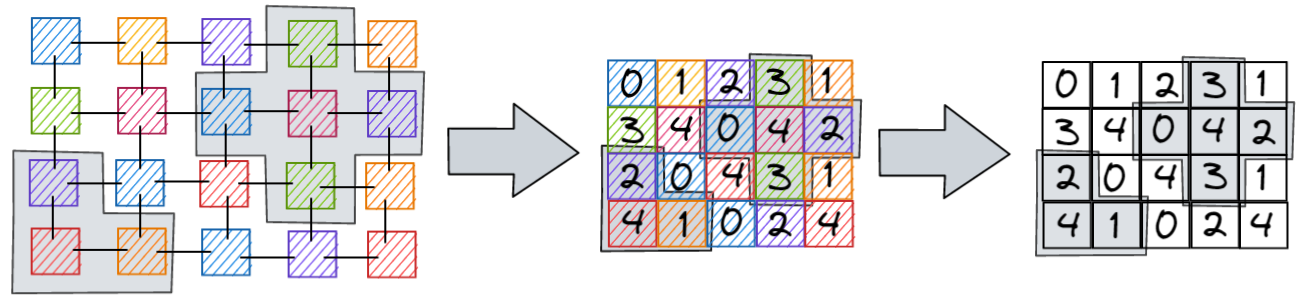
\includegraphics[width=1\textwidth]{Imagenes/ACaMatriz.PNG}
  \caption{Implementación computacional clásica de un autómata celular}
  \label{fig:AC a matriz}
\end{figure}
\end{frame}

\begin{frame}{Autómatas Celulares}
\begin{itemize}
    \item Un espacio discreto $\mathcal{L}$ regular en el que se encuentran todas las células.
    \item Un conjunto finito $\Sigma$ de todos los posibles valores que pueda adquirir una célula.
    \item Un sistema de vecindades que defina una topología sobre $\mathcal{L}$. Usualmente se define explícitamente la vecindad que se considera para todas las células.
    \item Una regla de evolución $\phi:\overbrace{\Sigma\times\Sigma\times\cdots\times\Sigma}^{N}\to\Sigma$ que define el cambio entre los $N$ posibles estados para una célula.
    \item Las condiciones de frontera para el espacio $\mathcal{L}$. De acuerdo con \cite{ACaplicacionesComputacion}, se consideran tres tipos de bordes: 
    \begin{itemize}
        \item \textbf{Bordes periódicos:} Las células opuestas son vecinas, es decir, $\mathcal{L}$ es un toro.
        \item \textbf{Bordes absorbentes:} Las células de los bordes no tienen vecinos fuera de los límites. En este caso $\mathcal{L}$ se puede entender como una región rectangular.
        \item \textbf{Bordes reflejantes:} Las células de los bordes tienen como vecinos fuera de los límites a la celda misma, formando una especie de espejo.
    \end{itemize}
    En nuestro caso trabajaremos solo con bordes del tipo absorbente.
\end{itemize}
\end{frame}

\begin{frame}{Autómatas Celulares}
La vecindad de Von neumann se compone de una célula central y de las que se encuentran a los lados formando así una especie de cruz:

$$\mathcal{V}_V(x_{i,j}) = \{x_{k,l}\mid\abs{i-k}+\abs{j-l}\leq1\text{, con }k,l\in\mathbb{Z}\}$$

La vecindad de Moore se define de manera similar a la vecindad de Von neumann, la diferencia entre una y otra radica en que la vecindad de Moore incluye a las células de las diagonales formando un cuadrado:

$$\mathcal{V}_M(x_{i,j}) = \{x_{k,l}\mid\abs{i-k},\abs{j-l}\leq1\text{, con }k,l\in\mathbb{Z}\}$$

\begin{figure}[h]
  \centering
    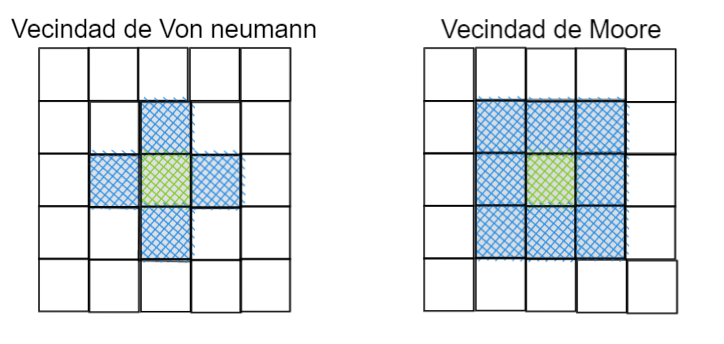
\includegraphics[width=0.5\textwidth]{Imagenes/vecindades.PNG}
  \caption{Vecindades usuales para autómatas celulares}
  \label{fig:Moore - Von neumann}
\end{figure}
\end{frame}

\begin{frame}{Autómatas Celulares}
Existen dos tipos de reglas de evolución para autómatas celulares, las determinísticas y las totalísticas. Las \textbf{reglas deterministicas} son aquellas en las que se determina un estado para cada posible configuración del vecindario, esto complica demasiado las cosas en un sistema de dos dimensiones, ya que podemos tener $5^{5^9}$ configuraciones para la vecindad de Moore y $5^{5^5}$ configuraciones para la vecindad de Von neumann \cite{ACaplicacionesComputacion}.

En el caso de las \textbf{reglas totalísticas} se definen los estados a partir de propiedades sobre las vecindades. Este tipo de regla facilita en gran medida la construcción de análisis sobre autómatas celulares, ya que se requiere de un menor almacenamiento en memoria para la cantidad de posibles casos.
\end{frame}

%\begin{frame}[allowframebreaks]{Referencias}
%\bibliographystyle{plain} % apalike
%\bibliography{BibliMSc}
%\end{frame}

\end{document}